\documentclass[a4paper,landscape]{foils}

\usepackage[pdftex,
        pdfauthor={Sara Fleury},
        pdfsubject={GenoM},
        pdftitle={GenoM},
        pdfkeywords={GenoM}]{hyperref}
\usepackage{mhfoils}
\usepackage{genom}
\usepackage{tabularx}
\usepackage{amssymb}

\setlength\topmargin{-2cm} 
\setlength\textheight{17cm} 

\graphicspath{{./figures/}}

\newcommand{\figw}[2]{
        \centerline{
	         \includegraphics[width=#2]{#1}
%%		\psfig{figure=#1,width=#2,clip=}
	}
}
\newcommand{\figc}[3]{
        \centerline{
\parbox{#2}{
	         \includegraphics[width=#2]{#1}\\
%%		\psfig{figure=#1,width=#2,clip=}
        \centerline{
		{\em\footnotesize #3}
		}
           }
	}
}

\MyLogo{{\color{darkyellow}http://softs.laas.fr/openrobots}}
%%\figw{./figures/openlaas.png}{1cm}}


\newcommand{\bi}{\begin{itemize}\itemsep 0mm}
\newcommand{\ei}{\end{itemize}}
\newcommand{\be}{\begin{enumerate}\itemsep 0mm}
\newcommand{\ee}{\end{enumerate}}
\newcommand{\bd}{\begin{description}\itemsep 0mm}
\newcommand{\ed}{\end{description}}

%-------------------------------------------------
\title{The Generator of Modules \\ \GenoM{}}
 
\author{Sara Fleury}
 
\date{July 2006\\[4cm]
\figw{./figures/openlaas.png}{4cm}}

%-------------------------------------------------


\begin{document}

\maketitle


%----------------------------------------------------------------------
\begin{tran}{Plan}

\begin{enumerate}
\itemsep 1mm
\item \bf General presentation %\rm  (p.2)
\item \bf How to write a module %\rm   (p.10)
\item \bf How to generate a module %\rm  (p.22)
\item \bf How to run a module %\rm  (p.32)
\item \bf How to integrate algorithms (codels) %\rm  (p.40)
\item \bf Codels and activities %\rm  (p.44)
\item \bf How to use a module %\rm  (p.55)
\item \bf Conclusions %\rm  (p.67)
\end{enumerate}

\end{tran}

%----------------------------------------------------------------------
\begin{tran}{\GenoM{} : Generator of Modules\label{gene}}

\begin{center}
\begin{tabularx}{\linewidth}{p{6cm}Xp{6cm}}
 \figc{adam-detour-web-small.jpg}{3.5cm}{adam} &
 \figc{junior-detour-web-small.jpg}{2.5cm}{junior} &
 \figc{lama-detour-web-small.jpg}{3.5cm}{lama} \\

 \figc{h2-detour-web-small.jpg}{4cm}{h2} &
 \figc{h2bis-detour-web-small.jpg}{3.2cm}{h2bis} &
 \figc{lapa-detour-web-small.jpg}{3cm}{lapa} \\

 \figc{karma-detour-web-small.jpg}{6cm}{karma} &
 \figc{diligent-detour-web-small.jpg}{1.7cm}{diligent} &
 \figc{scouts-detour-web-small.jpg}{2.1cm}{scout} \\
\end{tabularx}
\end{center}
\end{tran}

%----------------------------------------------------------------------
\begin{tran}{\GenoM{} : Generator of Modules\label{gene}}

\begin{center}
\begin{tabularx}{\linewidth}{p{6cm}Xp{6cm}}
 \figc{dala-detour-web-small.jpg}{3.1cm}{dala} &
 \figc{rackham-detour-web-small.jpg}{1.3cm}{rackham} &
 \figc{jidowanki-detour-web-small.jpg}{3.2cm}{jido} \\
{\centerline{\huge soon ?}}  & &\\
\figc{lhassa-detour-web-small.jpg}{4cm}{lhassa}
& \figc{hrp2.pdf}{2cm}{hrp2} & \figc{PatrolDX.jpg}{2cm}{Pioneer / Player} 
\end{tabularx}
\end{center}
\end{tran}

%----------------------------------------------------------------------
\begin{tran}{\GenoM{} : Generator of Modules\label{gene}}

Tool to integrate processing functions into independant servers or \textbf{modules}

\vspace{0.3cm}

\figw{./figures/module-simple}{11cm}

\textbf{Activity :} function in processing

\textbf{Reports :} �incorrect-parameters�, �solution-not-found�, 
�not-enough-memory�, �unforeseen-case�

\end{tran}

%----------------------------------------------------------------------
\begin{tran}{Why encapsulate functions ?}


\centerline{ \textbf{Software integration on embedded systems} }

 \textbf{Requirements :} 

	\begin{itemize}

	\item Controllable system
		\begin{itemize}

		\item processing start/stop
		\item dynamic parameterization
		\item error recovery
		\end{itemize}

	\item Communicating system
		\begin{itemize}
		\item data transfers
		\item use of other functions
		\end{itemize}
	\end{itemize}


\end{tran}

%----------------------------------------------------------------------
\begin{tran}{Why encapsulate functions (cont.)}

 \textbf{Requirements (cont.) } 


	\begin{itemize}
	\item Standard interfaces
		\begin{itemize}
		\item list of available functions
		\item Data structures of input/outputs
		\item Validity domains
		\item List of failure reports
		\end{itemize}

	\item Standard organization of files

	\end{itemize}

\end{tran}

%----------------------------------------------------------------------
\begin{tran}{Why encapsulate functions (cont.)}
 \textbf{Pros:}
\begin{description}
\item $\rightarrow$ makes integration simpler (semi-automatic)

\item $\rightarrow$ makes maintainance simpler (\textbf{sustainability}
and \textbf{perenity})
\end{description}

\textbf{Cons:}
\begin{description}
\item $\rightarrow$ Need to learn GenoM !
\end{description}

\end{tran}

%----------------------------------------------------------------------

\begin{tran}{Module creation principle}

\bd 
\item [4 steps:]~
      \begin{enumerate}
      \item Describe the module (\texttt{.gen} file):
	    \begin{itemize}
	    \item name
	    \item list of services (requests): parameters, functions, \ldots
	    \end{itemize}
      \item Generate the module (\texttt{genom})
      \item Incrementally fill-in algorithms
      \item Compile everything
      \end{enumerate}

\item [One gets: ]~
      \begin{itemize}
      \item one executable program: the module itself,
      \item libraries to communicate with the module,
      \item an interactive test program.
      \end{itemize}
\ed

\end{tran}

%----------------------------------------------------------------------
\begin{tran}{What can a module do ?}

\begin{itemize}
\item ``simple'' computations
\item device control
\item servoing
\item monitoring
\item use data produced by other modules
\end{itemize}

\end{tran}

%----------------------------------------------------------------------
\begin{tran}{Sample modules : Lama  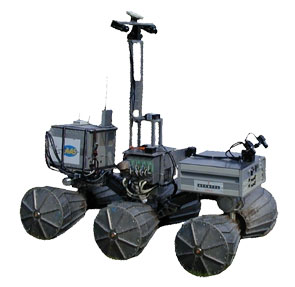
\includegraphics[width=1.8cm]{lama-detour-web-small.jpg}
}

\vspace{0.5cm}

\figw{./figures/lama-components-112002}{21cm}

\end{tran}

%----------------------------------------------------------------------
\begin{tran}{Sample modules : Karma  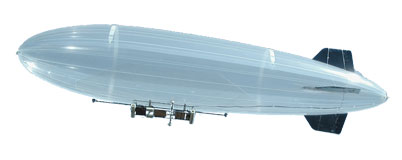
\includegraphics[width=3.5cm]{karma-detour-web-small.jpg}
}

\vspace{0.5cm}

\figw{karma-components.pdf}{21cm} 
\end{tran}

%----------------------------------------------------------------------
\begin{tran}{Sample modules : Rackham  
\includegraphics[width=0.5cm]{rackham-detour-web-small.jpg}
}

%\vspace{1cm}

\figw{rackham-components.png}{16cm} 

\end{tran}

%----------------------------------------------------------------------
\begin{tran}{How to communicate with a module?}

\textbf{Requests} (\texttt{msgLib}) \\

\figw{./figures/moduleRqst2}{17cm}

\begin{center} \textbf{$\rightarrow$ control flow} \end{center}
\end{tran}

%----------------------------------------------------------------------
\begin{tran}{How to communicate with a module?}

\textbf{Posters} (\texttt{posterLib})


\figw{./figures/modulePoster}{17cm}

\begin{center}  \textbf{$\rightarrow$ data flow}  \end{center}

\texttt{pocolibs} (\url{http://softs.laas.fr/openrobots})

\end{tran}


%----------------------------------------------------------------------
\begin{tran}{Behavior of a module: control request}

%%
%% METTRE LES FLECHES EN PARLANT
%%
\vspace{1cm}

\figw{./figures/module-fonctionmt}{10cm}

\end{tran}

%----------------------------------------------------------------------
\begin{tran}{Behavior of a module: execution request}

%%
%% METTRE LES FLECHES EN PARLANT
%%
\vspace{1cm}

\figw{./figures/module-fonctionmt2}{10cm}

\end{tran}


%----------------------------------------------------------------------
\begin{tran}{Development cycle of a module}

\vspace{1cm}

\figw{figures/cycle}{20cm}

7 steps (incling 4 ``transparent''):
\vspace{-0.5cm}
\begin{center}
\begin{tabularx}{\linewidth}{ll|X}
\bf 1. & \textbf{describe the module:} edit the \texttt{.gen} file, & \\
 2. \& 3. & generate + build the module (\texttt{make}), & iterate as
many times \\ 
\bf 4. & \textbf{write the algorithms} (codels), &  as needed. \\
 5. \& 6. & compile codels +  & \\
	& link edition with the module (\texttt{make}), & \\
\bf 7. & \textbf{test the module.} & 
\end{tabularx}
\end{center}


\end{tran}


%----------------------------------------------------------------------
%----------------------------------------------------------------------
\begin{tran}{\LARGE 2nd part : \\[7mm]Editing a module}\label{edition}

\begin{center}
{\em Summary of 1st part}
\end{center}

\begin{tabbing}
\textbf{Module : } \=
 database\\
 \> + processing functions  (set of \textbf{codels})\\
 \> + execution engine
\end{tabbing}

\textbf{Requests:} control and execution 

\textbf{Posters:} data transfers

\textbf{Activity:}  executing process of a request

\end{tran}
%----------------------------------------------------------------------

\begin{tran}{Directories setup}

\begin{itemize}
\item General configuration :

Openrobots tools installed in \verb|$prefix| (\texttt{/usr/local/openrobots}) 
%$

Environment variables:
\begin{itemize}
\item PATH \verb|$prefix/bin| %$
\item PKG\_CONFIG\_PATH \verb|$prefix/lib/pkgconfig| %$
\end{itemize}

\item  module directory for \texttt{demo}  :

\begin{tabular}{|l|ll|}
\hline
\texttt{demo/}  & description of the module  & \texttt{demo.gen} \\
		& description of structures  & \texttt{demoStruct.h} \\
\hline
\texttt{demo/server/}  & the server (generated by \GenoM{}) &\\
\hline
\texttt{demo/autoconf/} & the GNU autotools scripts &\\
\hline
\texttt{demo/codels/}  &  the algorithms (codels) & \tt demoXxxCodels.c\\
\hline
\end{tabular}

\end{itemize}

\end{tran}

%----------------------------------------------------------------------
\begin{tran}{Components of a module description}

The \texttt{demo.gen} file describes:

\begin{itemize}
\item module (name + identifier)
\item internal database (C structure)
\item requests 
\item posters
\item execution tasks
\end{itemize}

\end{tran}


%----------------------------------------------------------------------
\begin{tran}{Edition of the module \texttt{demo.gen} : emacs \texttt{genom} mode}

Configuration file \texttt{.emacs}
\vspace*{.5cm}
{\footnotesize
\begin{cartouche}
\begin{verbatim}
(setq load-path (cons "/usr/local/openrobots/genom/emacs"  load-path))
(setq auto-mode-alist (cons '("\\.gen$" . genom-mode) auto-mode-alist))
(autoload 'genom-mode "genom-mode" "Genom-mode" t)
\end{verbatim}
\end{cartouche}
}
%$

Commands (or menu) :

{\small
\begin{tabularx}{\linewidth}{|l|X|}
\hline
\tt C-c C-m & \textbf{m}odule creation ({\em 1st command to call})\\
\tt C-c C-i & \textbf{i}mportation de structures \\
\tt C-c C-r & \textbf{r}equest creation \\
\tt C-c C-p & \textbf{p}oster creation\\
\tt C-c C-e & \textbf{e}xecution task creation\\
\hline
\tt C-c C-b & \textbf{b}uffer indentation \\
\tt C-c C-v & \textbf{v}erify fields syntax \\
\tt C-c C-d & \textbf{d}elete unused fields \\
\hline
\tt C-c C-h \ldots & \textbf{h}elp on line\\
\hline
\end{tabularx}}


\end{tran}

%----------------------------------------------------------------------
\begin{tran}{A first module example}

How to control the motion of a mobile moving along one axis ?

\figw{figures/mobile}{12cm}


\begin{itemize}
\item {\bf One main service}: "move the mobile to a given position"\\
$\Rightarrow$ {\bf execution request}: \texttt{Goto}
%\vspace{-.8cm}
		\begin{itemize}
		\item input : \texttt{position} to reach
		\end{itemize}
\item {\bf parameters control}: "get or change speed reference"\\
	 $\Rightarrow$ {\bf control request}: 
		\begin{itemize}
		\item \texttt{SetSpeed} with input: new speed reference
		\item \texttt{GetSpeed} with output : current speed reference
		\end{itemize}
\end{itemize}
\end{tran}

%----------------------------------------------------------------------
\begin{tran}{Edition of \texttt{demo.gen}: module declaration}

%\vspace*{-0.3cm}
\textbf{\texttt{C-c C-m demo}}
%\vspace*{-0.2cm}
{\tiny
\begin{cartouche}
\begin{verbatim}
/*-------------------------------------------------------
 *               --  Module  DEMO  --
 *
 *  Description:       The only purpose is to do a demo
 *  Creation date:     Sat Jul 15 13:20:11 CEST 2006
 *  Author:            Sara Fleury
 *--------------------------------------------------------

module demo {
     number:          <<number>>;
     version:         "0.1";
     email:           <email>;
     requires:        <package-or-module> ...;
     internal_data:   DEMO_STR;
     uses_cxx:        0;
}; 

/*-------------------------------------------------------
 *               Structures and IDS
 *-------------------------------------------------------*/
#include "demoStruct.h"

typedef struct DEMOCAL_STR {

} DEMOCAL_STR;
\end{verbatim}
\end{cartouche}
}
\end{tran}

%----------------------------------------------------------------------
\begin{tran}{Edition of \texttt{demo.gen} : creation of a control request}
\vspace*{1cm}

{\footnotesize
\begin{cartouche}
\begin{verbatim}

/*--------------------------------------------------
 *             Requests 
 *--------------------------------------------------*/

request SetSpeed {
    doc:                  "<some doc>";
    type:                 control;
    input:                <name>::<sdi-ref>; 
    input_info:           <default-value>::"<doc>" , ...;
    output:               <name>::<sdi-ref>; 
    c_control_func:       demoSetSpeedCntrl;
    fail_msg:             <msg-name> , ...;
    incompatible_with:    <exec-rqst-name> , ...;
};
\end{verbatim}
\end{cartouche}
}
\end{tran}

%----------------------------------------------------------------------
\begin{tran}{Edition of \texttt{demo.gen} : creation of an execution request}
\vspace*{1cm}

{\small
\begin{cartouche}
\begin{verbatim}
request Goto {  
    doc:                  "<some doc>";
    type:                 exec;
    exec_task:            <<exec-task-name>>; 
    input:                <name>::<sdi-ref>; 
    input_info:           <default-value>::"<doc>" , ...;
    posters_input:        <struct-name>, ...;
    output:               <name>::<sdi-ref>; 
    c_control_func:       demoGotoCntrl;
    c_exec_func_start:    demoGotoStart; 
    c_exec_func:          demoGotoExec; 
    c_exec_func_end:      demoGotoEnd; 
    c_exec_func_inter:    demoGotoInter; 
    fail_msg:             <msg-name> , ...; 
    incompatible_with:    Goto, <exec-rqst-name>, ...; 
};
\end{verbatim}
\end{cartouche}
}
\end{tran}

%----------------------------------------------------------------------
\begin{tran}{Edition of \texttt{demo.gen}: creation of a poster}
\vspace*{1cm}

\begin{cartouche}
\begin{verbatim}
poster Status {
    update:              auto;
    data:                <<name>>::<<sdi-ref>> , ...;
    exec_task:           <<exec-task-name>>; 
};
\end{verbatim}
\end{cartouche}
\end{tran}

%----------------------------------------------------------------------
\begin{tran}{Edition of \texttt{demo.gen} : creation of an execution task}
\vspace*{1cm}

{\small
\begin{cartouche}
\begin{verbatim}
exec_task MotionTask {
    period:              <number>;
    delay:               <number>;
    priority:            <<number>>;
    stack_size:          <<number>>;
    c_init_func:         demoMotionTaskInit;
    c_func:              demoMotionTaskPerm;
    c_end_func:          demoMotionTaskEnd;
    fail_msg:            <msg-name> , ...;
};
\end{verbatim}
\end{cartouche}}

\end{tran}


%----------------------------------------------------------------------
\begin{tran}{Description of the module \texttt{demo.gen}}

{\footnotesize
\begin{cartouche}
\begin{verbatim}
/* ---- Module declaration ---- */
module demo {
     number:                9000;
     internal_data:         DEMO_STR;
     version:         "0.1";
     email:           sara@laas.fr;
     internal_data:   DEMO_STR;
     uses_cxx:        0;
};

/* ---- Structure definitions ---- */
#include "demoStruct.h"
#include "demoConst.h"

/* ---- Database of the module ---- */
typedef struct DEMO_STR {
     DEMO_STATE_STR state;         /* Current state */
     DEMO_SPEED     speedRef;      /* Speed reference */
     double         posRef;        /* Position reference */
     double         monitor;       /* Positions monitors */
}DEMO_STR;
\end{verbatim}
\end{cartouche}
}
\end{tran}

%----------------------------------------------------------------------
\begin{tran}{Description of the module \texttt{demo.gen} (cont.)}

%\vspace{1cm}

{\small
%\vspace{-1cm}
\begin{cartouche}
\begin{verbatim}
/* ---- declaration of the services: the requests ---- */

/* Control requests */
request SetSpeed {
    doc:                    "To change speed";
    type:                   control;
    input:                  speed::speedRef;
    input_info:             DEMO_DEFAULT_SPEED::"DEMO_SLOW or DEMO_FAST";
    c_control_func:         controlSpeed;
    fail_msg:               INVALID_SPEED;
};

request GetSpeed {
    doc:                    "To get current speed value";
    type:                   control;
    output:                 speed::speedRef;
};
\end{verbatim}
\end{cartouche}
}
\end{tran}

%----------------------------------------------------------------------
\begin{tran}{Description of the module \texttt{demo.gen} (cont. 2)}

%\vspace{1cm}

{\small
%\vspace{-1cm}
\begin{cartouche}
\begin{verbatim}
/* Execution requests */
request Goto {
    doc:                    "Goto the given position";
    type:                   exec;
    input:                  goal::posRef;
    input_info:             0::"position in m";
    c_control_func:         demoGotoCntrl;
    fail_msg:               TOO_FAR_AWAY;
    c_exec_func_start:      demoGotoStart;
    c_exec_func:            demoGotoExec;
    c_exec_func_end:        demoGotoEnd;
    c_exec_func_inter:      demoGotoEnd;
    incompatible_with:      Goto;
    exec_task:              MotionTask;
};
\end{verbatim}
\end{cartouche}
}

\end{tran}
%----------------------------------------------------------------------
\begin{tran}{Description of the module \texttt{demo}: structures and constants}

{\footnotesize
\begin{cartouche}
\begin{verbatim}
#ifndef DEMO_STRUCT_H
#define DEMO_STRUCT_H

typedef struct DEMO_STATE_STR {
  double position;  /* currente position (m) */
  double speed;     /* current speed (m/s) */
} DEMO_STATE_STR;

typedef enum DEMO_SPEED {
  DEMO_SLOW, 
  DEMO_FAST
}DEMO_SPEED;
\end{verbatim}
\end{cartouche}
}
\vspace{0.3cm}

{\footnotesize
\begin{cartouche}
\begin{verbatim}
#ifndef DEMO_CONST_H
#define DEMO_CONST_H

#define DEMO_MACHINE_LENGTH    20.0       /* m */
#define DEMO_DEFAULT_SPEED     DEMO_FAST  /* DEMO_SLOW */

#endif
\end{verbatim}
\end{cartouche}
}

\end{tran}

%----------------------------------------------------------------------
%----------------------------------------------------------------------
\begin{tran}{\Large 3rd part: \\[7mm]Generation and compilation}

\begin{center}
{\em Summary of 2nd part}
\end{center}

3 files to describe a module:
\vspace*{-.8cm}
	\begin{itemize}
	\itemsep -.5cm
	\item description file \texttt{demo.gen}
	\item structures \texttt{demoStruct.h}
	\item constants \texttt{demoConst.h}
	\end{itemize}
\vspace*{-.6cm}

5 parts in the  \textbf{.gen} file:
\vspace*{-.8cm}
	\begin{itemize}
	\itemsep -.5cm
	\item module (name + identifier)
	\item database (data structures)
	\item requests
	\item posters
	\item execution tasks
	\end{itemize}

\end{tran}
%----------------------------------------------------------------------
\begin{tran}{First generation of the module : \texttt{genom demo.gen}}

%\vspace{0.1cm}

%Commande : \texttt{genom -i demo.gen}

{\tiny
\begin{cartouche}
\begin{verbatim}
blues% genom demo.gen
genom demo.gen: info: array MonitorInput added in SDI for request Monitor
genom demo.gen: info: array MonitorOutput added in SDI for request Monitor
perl -w ./demo.pl

Updating top directory
  creating autogen

Updating codels
  demoMotionTaskCodels.c changed, skipping
  demoCntrlTaskCodels.c changed, skipping
  Makefile.in changed, skipping

Updating autoconf
  creating genom.mk
...
Updating server
  creating Makefile.in
...
Creating build environment ...
  * Running aclocal
  * Running autoconf

If you already have a build of this module, do not forget to
reconfigure (for instance by running ./config.status --recheck)

Done.
\end{verbatim}
\end{cartouche}
}
\end{tran}

\begin{tran}{GenoM outputs}

Production of several files and directories :
%\vspace{-1cm}
\begin{itemize}
\itemsep -0.2cm
\item \texttt{Makefile.in}, \texttt{configure}...
\item \texttt{server/}, \texttt{autoconf} and \texttt{codels/}
\end{itemize}

{\footnotesize
\begin{cartouche}
\begin{verbatim}
autogen*            configure.ac.user   local.mk.in 
Makefile.in         demo.gen            server/
acinclude.user.m4   codels/             demoConst.h         
autoconf/           configure*          demoStruct.h        
\end{verbatim}
\end{cartouche}
}

\end{tran}
%----------------------------------------------------------------------
\begin{tran}{GenoM outputs: the server}


In \texttt{demo/server/} files used by genom and clients of the module, related to:
\begin{itemize}
\item server : 
	\texttt{demoCntrlTask, demoMotionTask, \ldots}
\item libraries to send requests and receive replies
	\texttt{demoMsgLib}
\item libraries to access posters:
	\texttt{demoPosterLib}
\item Test program :
	\texttt{demoTest.c}
\end{itemize}
\end{tran}
%----------------------------------------------------------------------
\begin{tran}{GenoM outputs: codels}

In \texttt{demo/codels/}
files that will contain the algorithms.

1 codels file per task:

\begin{itemize}
\item Control codels:
 \texttt{democCntrlTaskCodels.c}
\item Execution codels:
 \texttt{demoMotionTaskCodels.c}
\item Autoconf infrastructure:
\texttt{Makefile.in} \texttt{autoconf/} \texttt{configure}
\end{itemize}

\end{tran}

%----------------------------------------------------------------------
\begin{tran}{Configurating the module}

Create a build directory:

{\tiny
\begin{cartouche}
\begin{verbatim}
blues% mkdir build
blues% cd build
\end{verbatim}
\end{cartouche}}

Call configure, telling where to install the module:

{\tiny
\begin{cartouche}
\begin{verbatim}
blues% ../configure --prefix=/usr/local/openrobots
checking build system type... i686-pc-linux-gnu
checking host system type... i686-pc-linux-gnu
checking for gcc... gcc
checking for C compiler default output file name... a.out
...
config.status: creating codels/Makefile
config.status: creating server/Makefile
config.status: creating demo.pc
config.status: creating local.mk
\end{verbatim}
\end{cartouche}}
\end{tran}
%----------------------------------------------------------------------
\begin{tran}{Building the module}

Call: \texttt{make}

\begin{itemize}
\item re-generates the module if needed
\item builds everything
\end{itemize}

{\tiny
\begin{cartouche}
\begin{verbatim}
blues% make
make all-posix
make[1]: Entering directory `/usr/local/openrobots/modules/demo/build'
make[2]: Entering directory `/usr/local/openrobots/modules/demo/build/server'
mkdir -p posix-build
/usr/local/openrobots/i386-linux/bin/mkdep -c"gcc" -oposix-build/dependencies -dposix-build -t.lo -DUNIX    -I. -I../.. -I../../server -I/usr/local/openrobots/i386-linux/include   ../../server/demoCntrlTask.c ../../server/demoModuleInit
...
s/i386-linux/lib
creating posix-build/demo
make[2]: Leaving directory `/usr/local/openrobots/modules/demo/build/codels'
make[1]: Leaving directory `/usr/local/openrobots/modules/demo/build'
\end{verbatim}
\end{cartouche}}

\end{tran}

%----------------------------------------------------------------------
\begin{tran}{Installation}
The module needs to be installed to be useful.

{\small
\begin{cartouche}
\begin{verbatim}
blues% make install
\end{verbatim}
\end{cartouche}}

It is installed as specify with the \texttt{--prefix} option of \texttt{configure}.

According to the destination you have chosen, you may need \texttt{root} priviledges.
\end{tran}
%----------------------------------------------------------------------
%----------------------------------------------------------------------
\begin{tran}{\Large 4th part: \\[7mm]Execution}

\begin{center}
{\em Summary of 3rd part}
\end{center}

\begin{enumerate}
\item Edit the module : {\bf demo.gen}

\item Only the first time: generate {\bf genom} and configure {\bf configure}

\item Compile and generate : {\bf gnumake}

\item Install : {\bf gnumake install}

\end{enumerate}

\end{tran}

%----------------------------------------------------------------------
\begin{tran}{UNIX session : execution}


1. Start the communication server :

\begin{cartouche}
\begin{verbatim}
%blues h2 init
\end{verbatim}
\end{cartouche}

2. Start the module :

\begin{cartouche}
\begin{verbatim}
%blues demo -b
\end{verbatim}
\end{cartouche}

\texttt{-b} option allows to wait until the module has effectively
started.

3. Start the client(s) :

\begin{cartouche}
\begin{verbatim}
%blues demoTest 1
\end{verbatim}
\end{cartouche}

\end{tran}


%----------------------------------------------------------------------
\begin{tran}{The test program \texttt{demoTest} }

\figw{./figures/essay1}{11cm}

\end{tran}

%----------------------------------------------------------------------
\begin{tran}{The test program \texttt{demoTest} (cont) }

\vspace{2cm}

\figw{./figures/essay2}{8cm}

\end{tran}

%----------------------------------------------------------------------
\begin{tran}{UNIX  session : end}

1. Kill the module :

\begin{cartouche}
\begin{verbatim} 
%blues killmodule demo
\end{verbatim}
\end{cartouche}

or with the command \texttt{-99} in the \texttt{demoTest} menu.


{\bf (then one can restart the module)}

2. session ending :

\begin{cartouche}
\begin{verbatim} 
%blues h2 end
\end{verbatim}
\end{cartouche}

\end{tran}

%----------------------------------------------------------------------
%----------------------------------------------------------------------
\begin{tran}{\Large 5th part : \\[7mm]The codels}

\begin{center}
{\em Summary of 4th part}
\end{center}

\begin{enumerate}
\item Edit the module : {\bf demo.gen}

\item Only the first time: generate ({\bf genom}) and configure ({\bf configure})

\item (Re) generate and compile: {\bf make}

\item Install : {\bf make install}

\item Execute : {\bf h2 init, demo -b, demoTest 1, ... h2 end}

\end{enumerate}

\end{tran}

%----------------------------------------------------------------------
\begin{tran}{Codels}

\bi

\item All the codels are in the directory : {\tt codels/}

\item In this directory we have one codels file per task.

\item Thus for the \texttt{demo} we have:

\begin{itemize}
\item {\tt demoCntrlTaskCodels.c} for the control codels ({\tt c\_control\_func})

\item {\tt demoMotionTaskCodels.c} for the execution codels ({\tt
c\_exec\_func}, \ldots)

\end{itemize}
\end{itemize}
\end{tran}

%----------------------------------------------------------------------
\begin{tran}{Control codels}

{\footnotesize
\begin{cartouche}
\begin{verbatim}
STATUS demoSetSpeedCntrl(DEMO_SPEED *speed, int *report)
{
   /* Refuse *speed if the value is erroneous */
   if (*speed != DEMO_SLOW && *speed != DEMO_FAST) {
        *report = S_demo_INVALID_PARAMETER;
        return ERROR;
   }
   /* Parameter is valid: it will be recorded into the fIDS */
   return OK;
}

STATUS demoGotoCntrl(double *posRef, int *report)
{
   /* Refuse *posRef if the value is erroneous */
   if (fabs(*posRef) > DEMO_MCHINE_LENGTH/2.0) {
        *report = S_demo_INVALID_PARAMETER;
        return ERROR;
   }
   /* Parameter is valid: it will be recorded into the fIDS 
      and Goto request will start */
   return OK;
}
\end{verbatim}
\end{cartouche}}

\end{tran}


%----------------------------------------------------------------------
\begin{tran}{Execution codels}

{\footnotesize
\begin{cartouche}
\begin{verbatim}
ACTIVITY_EVENT demoGotoStart(double *posRef, int *report)
{
   printf("Start engin\n");
   return EXEC;
}

ACTIVITY_EVENT demoGotoExec(double *posRef, int *report)
{
   double dist = *posRef - SDI_f->state.position;
   switch(SDI_f->speedRef) {
       case DEMO_SLOW:
	    if (fabs(dist) < 0.1) return END;
	    SDI_f->state.position += sign(dist) * 0.1;
	    return EXEC;
       case DEMO_FAST:
	    if (fabs(dist) < 1) return END;
	    SDI_f->state.position += sign(dist) * 1;
	    return EXEC;
   }
}
\end{verbatim}
\end{cartouche}}

\end{tran}


%----------------------------------------------------------------------
\begin{tran}{Execution codels (cont)}

{\footnotesize
\begin{cartouche}
\begin{verbatim}
ACTIVITY_EVENT demoGotoEnd(double *posRef, int *report)
{
   SDI_f->state.position = *posRef;
   printf("Stop engin\n");
   return ETHER;
}
\end{verbatim}
\end{cartouche}}
\end{tran}


%----------------------------------------------------------------------
\begin{tran}{Particular codels}

\bi
\item Initialisation codel {\tt c\_init\_func} 

\item Terminaison codel  {\tt c\_end\_func} 

\item Permanent activity codel  : {\tt c\_func}
\ei

$\rightarrow$ one per execution task  \\

{\footnotesize
\begin{cartouche}
\begin{verbatim}
#include "demoConst.h"

STATUS demoComputeInit(int *report)
{
  SDI_F->state.position = 0.0;
  SDI_F->state.speed = 0.0;
  SDI_F->posRef = 0.0
  SDI_F->speedRef = DEMO_SLOW
  return OK;
}
\end{verbatim}
\end{cartouche}}

\end{tran}

%----------------------------------------------------------------------
%----------------------------------------------------------------------
\begin{tran}{\Large 6th part : \\[7mm]Codels and activities}

\begin{center}
{\em Summary of 5th part}
\end{center}

\begin{enumerate}
\item Edit the module : {\bf demo.gen}

\item Only the first time: generate ({\bf genom}) and configure ({\bf configure})

\item (Re) generate and compile: {\bf make}

\item Install : {\bf make install}

\item Execute : {\bf h2 init, demo -b, demoTest 1, ... h2 end}

\item Fill-in the codels (and goto {\bf 3})

\end{enumerate}

\end{tran}

%----------------------------------------------------------------------
\begin{tran}{Activities and codels}

\bi
\item generaly
1 activity $\rightarrow$ a sequence of codels :

{\tt start}\\
{\tt exec}\\
{\tt exec}\\
{\tt \ldots}\\
{\tt exec}\\
{\tt end}
\ei


\bi
\item Codels are not interruptible
\item Activity are interruptible on transitions between 2 codels.
\item On Interruption $\Rightarrow$ execution of the codel {\tt inter}
\ei 


\end{tran}


%----------------------------------------------------------------------
\begin{tran}{Execution requests and codels}

One example :

{\small
\begin{cartouche}
\begin{verbatim}
/* Translation on a given distance */
request Goto {
   type:                exec;               
   input:               distance::distRef;  
   c_control_func:      demoGotoCntrl;
   fail_msg:            TOO_FAR_AWAY;       
   c_exec_func_start:   demoGotoStart;     
   c_exec_func:         demoGotoExec;   
   c_exec_func_end:     demoGotoEnd;      
   c_exec_func_inter:   demoGotoInter;      
   incompatible_with:   Goto;       
   exec_task:           MotionTask;         
};
\end{verbatim}
\end{cartouche}
}

\end{tran}

%----------------------------------------------------------------------
\begin{tran}{Activities decomposition in codels}
\vspace{.5cm}

\fig{figures/grapheExec}{6cm}

\vspace{.1cm}
{\footnotesize
\begin{tabularx}{\linewidth}{|l|l|X|}
\hline
�tat 	 	& codel (if exists)	&  \\
\hline
\tt START  & \tt c\_exec\_func\_start  	& starting	\\
\tt EXEC   & \tt c\_exec\_func  	& main \\
\tt END    &\tt c\_exec\_func\_end 	& terminating \\
\tt FAIL   & \tt c\_exec\_func\_fail 	& terminating (pb) \\
\hline
\tt INTER  & \tt c\_exec\_func\_inter  	& terminating (on interruption) \\
\hline
\tt SLEEP  & 				& wait event \\
\tt ETHER    &	& \em activity over   \\
\tt ZOMBIE   &	& \em activity suspended  \\
\hline
\end{tabularx}}
\vspace{.1cm}

\end{tran}


%----------------------------------------------------------------------
\begin{tran}{Periodical task}

$\rightarrow$ Periodical task \\

\begin{cartouche}
\begin{verbatim}
exec_task Compute {
    period:                10;     /* 100ms */
    priority:              20;     /* a hight priority */
    stack_size:            10000;
};
\end{verbatim}
\end{cartouche}

\bi
\item usely 1 tic = 10ms on non-real-time unix
\item priority: [0..255] (0: higher priority): used only on real-time OS
\item stack\_sike: used only on real-time OS
\ei

\end{tran}

%----------------------------------------------------------------------
\begin{tran}{The posters : automatics or manual}

Exporte results

\bi

\item Automatical update every time its execution task wakes up

{\small
\begin{cartouche}
\begin{verbatim}
poster Status {
    update:              auto;
    data:                state::state;
    exec_task:           MotionTask;
};
\end{verbatim}
\end{cartouche}
}

\item Manual update only when necessary

{\small
\begin{cartouche}
\begin{verbatim}
poster Status {
    update:              user;
    type:                SPEED_REF;
    exec_task:           MotionTask;
};
\end{verbatim}
\end{cartouche}
}
\ei 

\end{tran}

%----------------------------------------------------------------------
\begin{tran}{Posters :  manual update}
Update from a codel : \\

{\footnotesize
\begin{cartouche}
\begin{verbatim}
ACTIVITY_EVENT demoGotoStart(double *posRef, int *report)
{
   printf("Start engin\n");
   if (demoStatusSPEED_REFPosterWrite 
                         (DEMO_STATUS_POSTER_ID,
                          SDI_F->speedRef) != OK) {
    *report = S_demo_CANNOT_WRITE_POSTER;
    return ETHER;
  }
   return EXEC;
}

\end{verbatim}
\end{cartouche}
}

\end{tran}

%----------------------------------------------------------------------
%----------------------------------------------------------------------
\begin{tran}{\Large 7th part : \\[7mm]Modules utilization}

\begin{center}
{\em Summary of 6th part}
\end{center}

\begin{enumerate}
\item Edit the module : {\bf demo.gen}

\item Only the first time: generate ({\bf genom}) and configure ({\bf configure})

\item (Re) generate and compile: {\bf make}

\item Install : {\bf make install}

\item Execute : {\bf h2 init, demo -b, demoTest 1, ... h2 end}

\item Fill-in the codels (and goto {\bf 3})

\end{enumerate}

\end{tran}
%----------------------------------------------------------------------
\begin{tran}{Using module structures from another module}

Import structures : 

{\small
\begin{cartouche}
\begin{verbatim}
module pilo {
     number:          9000;
     version:         "0.1";
     requires:        demo;
     internal_data:   PILO_STR;
}; 

import from demo {
#include "demoStruct.h"
};
#include "piloStruct.h"

typedef struct PILO_STR {
     PILO_GOTO_STR goto;
     DEMO_POS_REF  posRef;
} PILO_STR;
\end{verbatim}
\end{cartouche}
}

Based on \texttt{package config}.

\end{tran}

%----------------------------------------------------------------------
\begin{tran}{Read a poster from another module}

{\tiny
\begin{cartouche}
\begin{verbatim}
request Track {
   type:   exec;
   ...
   posters_input:    LOCO_SPEED_REF;
   ...
};
\end{verbatim}
\end{cartouche}
}

Library : {\tt demoPosterReadLib}

{\tiny
\begin{cartouche}
\begin{verbatim}
  POSTER_ID trackPosterId=-1;
  DEMO_REF ref;

  /* look for the poster */
  if (posterFind(track->posterName, &trackPosterId) == ERROR) {
    *report = S_demo_CANNOT_FIND_POSTER;
    return ETHER;
  }
  /* try to read the data for the first time */
  if (demoDEMO_REFPosterRead(trackPosterId, &ref) == ERROR) {
    *report = S_demo_CANNOT_READ_POSTER;
    return ETHER;
  }
...
\end{verbatim}
\end{cartouche}
}

\end{tran}

%----------------------------------------------------------------------
\begin{tran}{Control of a module with tclServ : principle}


\begin{itemize}
\item {\tt tclServ} allows to control a set of modules from a unique interface

\item Full interactive programming language  (tcl)

\item ASCII data transfert (non sensitive to data representation like little endian / big endian / alignment).

\item Graphical libraries {\tt tk}
\end{itemize}

{\tt  http://softs.laas.fr/openrobots/eltclsh}


\end{tran}
%----------------------------------------------------------------------
\begin{tran}{Module control with tclServ : using}

\begin{enumerate}
\item Generate the module with option {\tt -t}

\item Start the server {\tt tclserv}.

\item Start one (or several) tcl-shells :
{\tt eltclsh -package genom}

{\em Remark : make an alias !}

\item Start session (see example).

\end{enumerate}

\end{tran}
%----------------------------------------------------------------------
\begin{tran}{Module control with tclServ : options and commands}
\vspace{1cm}
{\center
{\small
\begin{tabularx}{\linewidth}{|l|X|}
\hline
option		& function \\
\hline
\tt -ack & non blocking request sending \\

\tt -raw & the result is presented as a raw list of data
           (not a nice display)  \\
\hline
command		& function \\
\hline
\tt replyof \$rqstId & get answer {\em blocking mode}. 
Generaly used with option {\tt -raw}. \\
\tt cs::term \$rqstId 0 & get answer {\em  non blocking mode}. \\
\tt abort \$rqstId	& abort the request \\
\tt kill $<$module$>$	& abort the module $<$module$>$ \\
\hline
\end{tabularx}}
}


\end{tran}

%----------------------------------------------------------------------
\begin{tran}{Module control with tclServ : examples}

{\footnotesize
\begin{cartouche}
\begin{verbatim}
tcl-> connect cabby
no startup script for cabby: Rack inconnu
sourcing ~/.tclservrc
connected to cabby
tcl[cabby]-> lm camera
camera loaded on cabby
tcl[cabby]-> lm platine
platine loaded on cabby
tcl[cabby]-> mboxInit 
csLib mailbox created on cabby
tcl[cabby]-> camera::Init
Working mode [CAMERA_LIVE] : 
Preprocessings mode [CAMERA_ENABLE_PREPROCESSINGS] : 
status = OK
tcl[cabby]-> 
\end{verbatim}
\end{cartouche}
}

{\small
\begin{cartouche}
\begin{verbatim}
    set demFused [dem::FuseDem -ack]
    set classifDone [lclassif::Classif -ack]
    replyof \$demFused
\end{verbatim}
\end{cartouche}
}

\end{tran}

%----------------------------------------------------------------------
\begin{tran}{Module control with tclServ : rackTab, tk, \ldots}

\begin{itemize}
\itemsep -0.3cm
\item Initialization file : {\tt .tclservrc}

\item Utilisation with {\tt rackTab} : option {\tt eltclsh -package rackTab} \\

\item Graphics tools with {\tt tk} : 

Two modular and extensibles graphical interfaces :
\begin{itemize}
\itemsep -0.2cm
\item 2D version: {\tt /usr/local/robots/grh2/}
\item 3D version: {\tt  http://softs.laas.fr/openrobots/gdhe.php}
\end{itemize}

All our robots have their 3D model (lama, h2, h2bis with son bras, diligent,
scouts). 

\end{itemize}

\end{tran}
%----------------------------------------------------------------------
\begin{tran}{Display with GDHE \ldots}

{\tt  http://softs.laas.fr/openrobots/tools/gdhe.php}

\fig{./figures/gdhe-robots.png}{10cm}


\end{tran}

%----------------------------------------------------------------------
\begin{tran}{Module control with OpenPRS : principle}

{\tt  http://softs.laas.fr/openrobots/tools/openprs.php}

\begin{itemize}
\item Supervision
\item Generate the module with option {\tt -o}
\end{itemize}

OPs producted for each request :

\vspace{.3cm}
{\center
{\small
\begin{tabularx}{\linewidth}{|l|X|}
\hline
nom		& function \\
\hline
\tt DEMO-MOTION & send the request  {\em and} receive the {\em
                    finale reply in blocking mode} \\

\tt DEMO-MOTION-REPORT & idem with the report  \\

\tt DEMO-MOTION-ASYNC & send the request in non blocking mode. \\

\hline
\end{tabularx}}
}

The answer is a string in the data base :
\\
{\tt (FR DEMO DEMO\_MOTION \$RQST-ID \$REPORT \$DATA)}.

\end{tran}

%----------------------------------------------------------------------
\begin{tran}{Module control with OpenPRS : {\tt transGen}}

\begin{itemize}
\item Automatic production of OpenPRS relocatable.
\item Similar to GenoM :

\begin{itemize}
\item  Description  file {\tt manip.tg} :
\end{itemize}


{\small
\begin{cartouche}
\begin{verbatim}
/* --- Declaration of a supervisor --- */
supervisor manip {
  module: xr4000;
  module: sick;
  module: m2d;
  module: segloc;
}
\end{verbatim}
\end{cartouche}
}

\end{itemize}

\end{tran}

%----------------------------------------------------------------------
\begin{tran}{Module control with OpenPRS : {\tt transGen} (continued)}

\begin{description}
\item ~
\begin{description}
\item - Call : {\tt tranGen manip.tg}
\item - Compile in {\tt server/}.
\item - Satrt OpenPRS : 
\end{description}

{\footnotesize
\begin{cartouche}
\begin{verbatim}
idefix[manip] server/i386-linux/manip-xOpenPRS -n manip-cabby 
-x server/data/manip-data.inc -x data/my-data.inc &
\end{verbatim}
\end{cartouche}
}

\end{description}

\end{tran}

%----------------------------------------------------------------------
\begin{tran}{Module control with OpenPRS : Example of procedure ({\tt OP})}

An OP taht starts
automatically the continuous 
localization request  ({\tt SEGLOC-LOCLOOP-ASYNC}) when the
robot losts itself  :

{\tiny
\begin{cartouche}
\begin{verbatim}
;;;;;;;;;;;;;;;;;;;;;;;;;
;;; |Localize|
;;;;;;;;;;;;;;;;;;;;;;;;;
(defop |Localize|
    :invocation (! (EXECUTE LOC-LOOP))
    :context (& (UNCERTAINTY-LEVEL-1 $X1 $Y1 $T1) 
                (ALARM-LEVEL-1 $L1))
    :body ((IF (! (EXECUTE LOC-LOCAL))
              (! (SPEAK "ok"))
              (! (SEGLOC-LOCLOOP-ASYNC $RQST-ID1))
              (! (CURRENT-MISSION-COMPLETED))
            ELSE
              (! (SPEAK "Bad localization. Try again"))
              (! (FAILED))
           )
          )
)
\end{verbatim}
\end{cartouche}
}
%$
\end{tran}

%----------------------------------------------------------------------
%----------------------------------------------------------------------
\begin{tran}{\Large Conclusion}

\begin{enumerate}
\item Edit the module : {\bf demo.gen}

\item Only the first time: generate ({\bf genom}) and configure ({\bf configure})

\item (Re) generate and compile: {\bf make}

\item Install : {\bf make install}

\item Execute : {\bf h2 init, demo -b, demoTest 1, ... h2 end}

\item Control with : {\bf tclserv} and {\bf tcl/tk} {\tt (eltclsh, elwish,
gdhe)}\\
	or {\bf OpenPRS}

\end{enumerate}

\end{tran}

%----------------------------------------------------------------------
\begin{tran}{On line documents}

Official page (not up-to-date !):
{\tt http://softs.laas.fr/openrobots}

Very usefull page by Roland Philippsen:
{\tt http://www.laas.fr/~rolo/openrobots-start.html}

Mailling-list: {\tt openrobots.laas.fr}

(Intranet) Wiki: 
{\tt http:/intranet.laas.fr/robots/wiki}

\end{tran}

\end{document}


\comment{
client init ...ok.   Poster init ...ok.
------------------------------------------------------------------------
  0: GetConstPoly          1: SetConstPoly          2: ComputePoly (E)
 
 55: posters   66: abort  77: replies (0)  88: state  99: QUIT  -99: END
------------------------------------------------------------------------
demo1 (88)> 0
 
(To abort type "a") 
 
** Final reply: OK
constPoly:
  a = 1.000000
  b = 2.000000
  c = 3.000000
 
------------------------------------------------------------------------
  0: GetConstPoly          1: SetConstPoly          2: ComputePoly (E)
 
 55: posters   66: abort  77: replies (0)  88: state  99: QUIT  -99: END
------------------------------------------------------------------------
demo1 (0)> 2
 
** Enter double xPoly: (0.000000) 2
Wait final reply (y/n/a) ? : y
 
** Final reply: OK
resPoly = 11.000000
 
------------------------------------------------------------------------
  0: GetConstPoly          1: SetConstPoly          2: ComputePoly (E)
 
 55: posters   66: abort  77: replies (0)  88: state  99: QUIT  -99: END
------------------------------------------------------------------------
demo1 (2)> 1
 
Get current constPoly using request GetConstPoly (y/n) ? (n) 
 
** Enter DEMO_CAL_CONST_POLY constPoly:
  a (0.000000) 
  b (0.000000) 1
  c (0.000000) 2
(To abort type "a") 
 
** Final reply: OK
 
------------------------------------------------------------------------
  0: GetConstPoly          1: SetConstPoly          2: ComputePoly (E)
 
 55: posters   66: abort  77: replies (0)  88: state  99: QUIT  -99: END
------------------------------------------------------------------------
demo1 (1)> 2
 
** Enter double xPoly: (2.000000) 
Wait final reply (y/n/a) ? : y
 
** Final reply: OK
resPoly = 4.000000
 
------------------------------------------------------------------------
  0: GetConstPoly          1: SetConstPoly          2: ComputePoly (E)
 
 55: posters   66: abort  77: replies (0)  88: state  99: QUIT  -99: END
------------------------------------------------------------------------
demo1 (2)> 
}


% LocalWords:  pdfsubject pdftitle pdfkeywords matthieu doc Fleury Herrb Codels
% LocalWords:  adam jpg bis lapa lama jidowanki rackham dala neobotix cont gen
% LocalWords:  genom pdf png msgLib moduleRqst posterLib modulePoster pocolibs
% LocalWords:  softs laas fr openrobots fonctionmt codels usr PKG ONFIG ATH cd
% LocalWords:  demoStruct autoconf autotools demoXxxCodels setq alist autoload
% LocalWords:  mkdir RQST
